\section{\gls{evse} Network}

For \gls{evse} networks, the nodes are charging stations. The focus of this document is long distance travel and , thus, only \gls{dcfc} nodes will be considered. Because interoperability between vehicles and chargers is not universal, the network will look different for different types of vehicle. An \gls{evse} network's links are ephemeral end vehicle-dependent. Links exist between all chargers and all other chargers within range. This creates a highly connected network with significant locality. A key feature of any \gls{evse} network is the low probability of availability at all nodes. Chargers are unreliable and may be unavailable for reasons including hardware and software faults, physical blockage, plug damage, payment system failures, and occupation. Because \gls{pev} fast charging events take a relatively long amount of time compared to \gls{icev} fueling events and the relatively low number of plugs per station and stations per mile of road network, the probability of plug occupation is high, especially for central nodes. This can lead to a frustrating driving experience as limited prior knowledge of charger availability is the norm.

Constructing an \gls{evse} network requires the locations of usable chargers, vehicle usable range, and a road network which has nodes coincident with the chargers, or nearly so. In this document, the road network will be referred to as the atlas. The links of the \gls{evse} network are constructed by finding the lowest cost (however defined) route for all node pairs which do not violate cost limits. Routing along the network involves the additional step of adding origins and destinations to the network in the same manner as adding chargers.

\subsection*{Random Graph}

Shown in Figure \ref{fig:random_graph} is a randomly generated graph ($G = \{V, E\}$) with a cardinality of $N = 100$ on a 100 km by 100 km area with a link probability determined by $P(E|L_E) = e^{-L / S}$ where $E$ is the link from $V_i$ to $V_j$, $L_E$ is the Pythagorean distance between $V_i$ and $V_j$, and $S$ is a characteristic distance, (10 km in this case). Among the nodes in the graph, one has been designated the origin, five have been assigned as destinations, and ten have been assigned as chargers.

\begin{figure}[H]
	\centering
	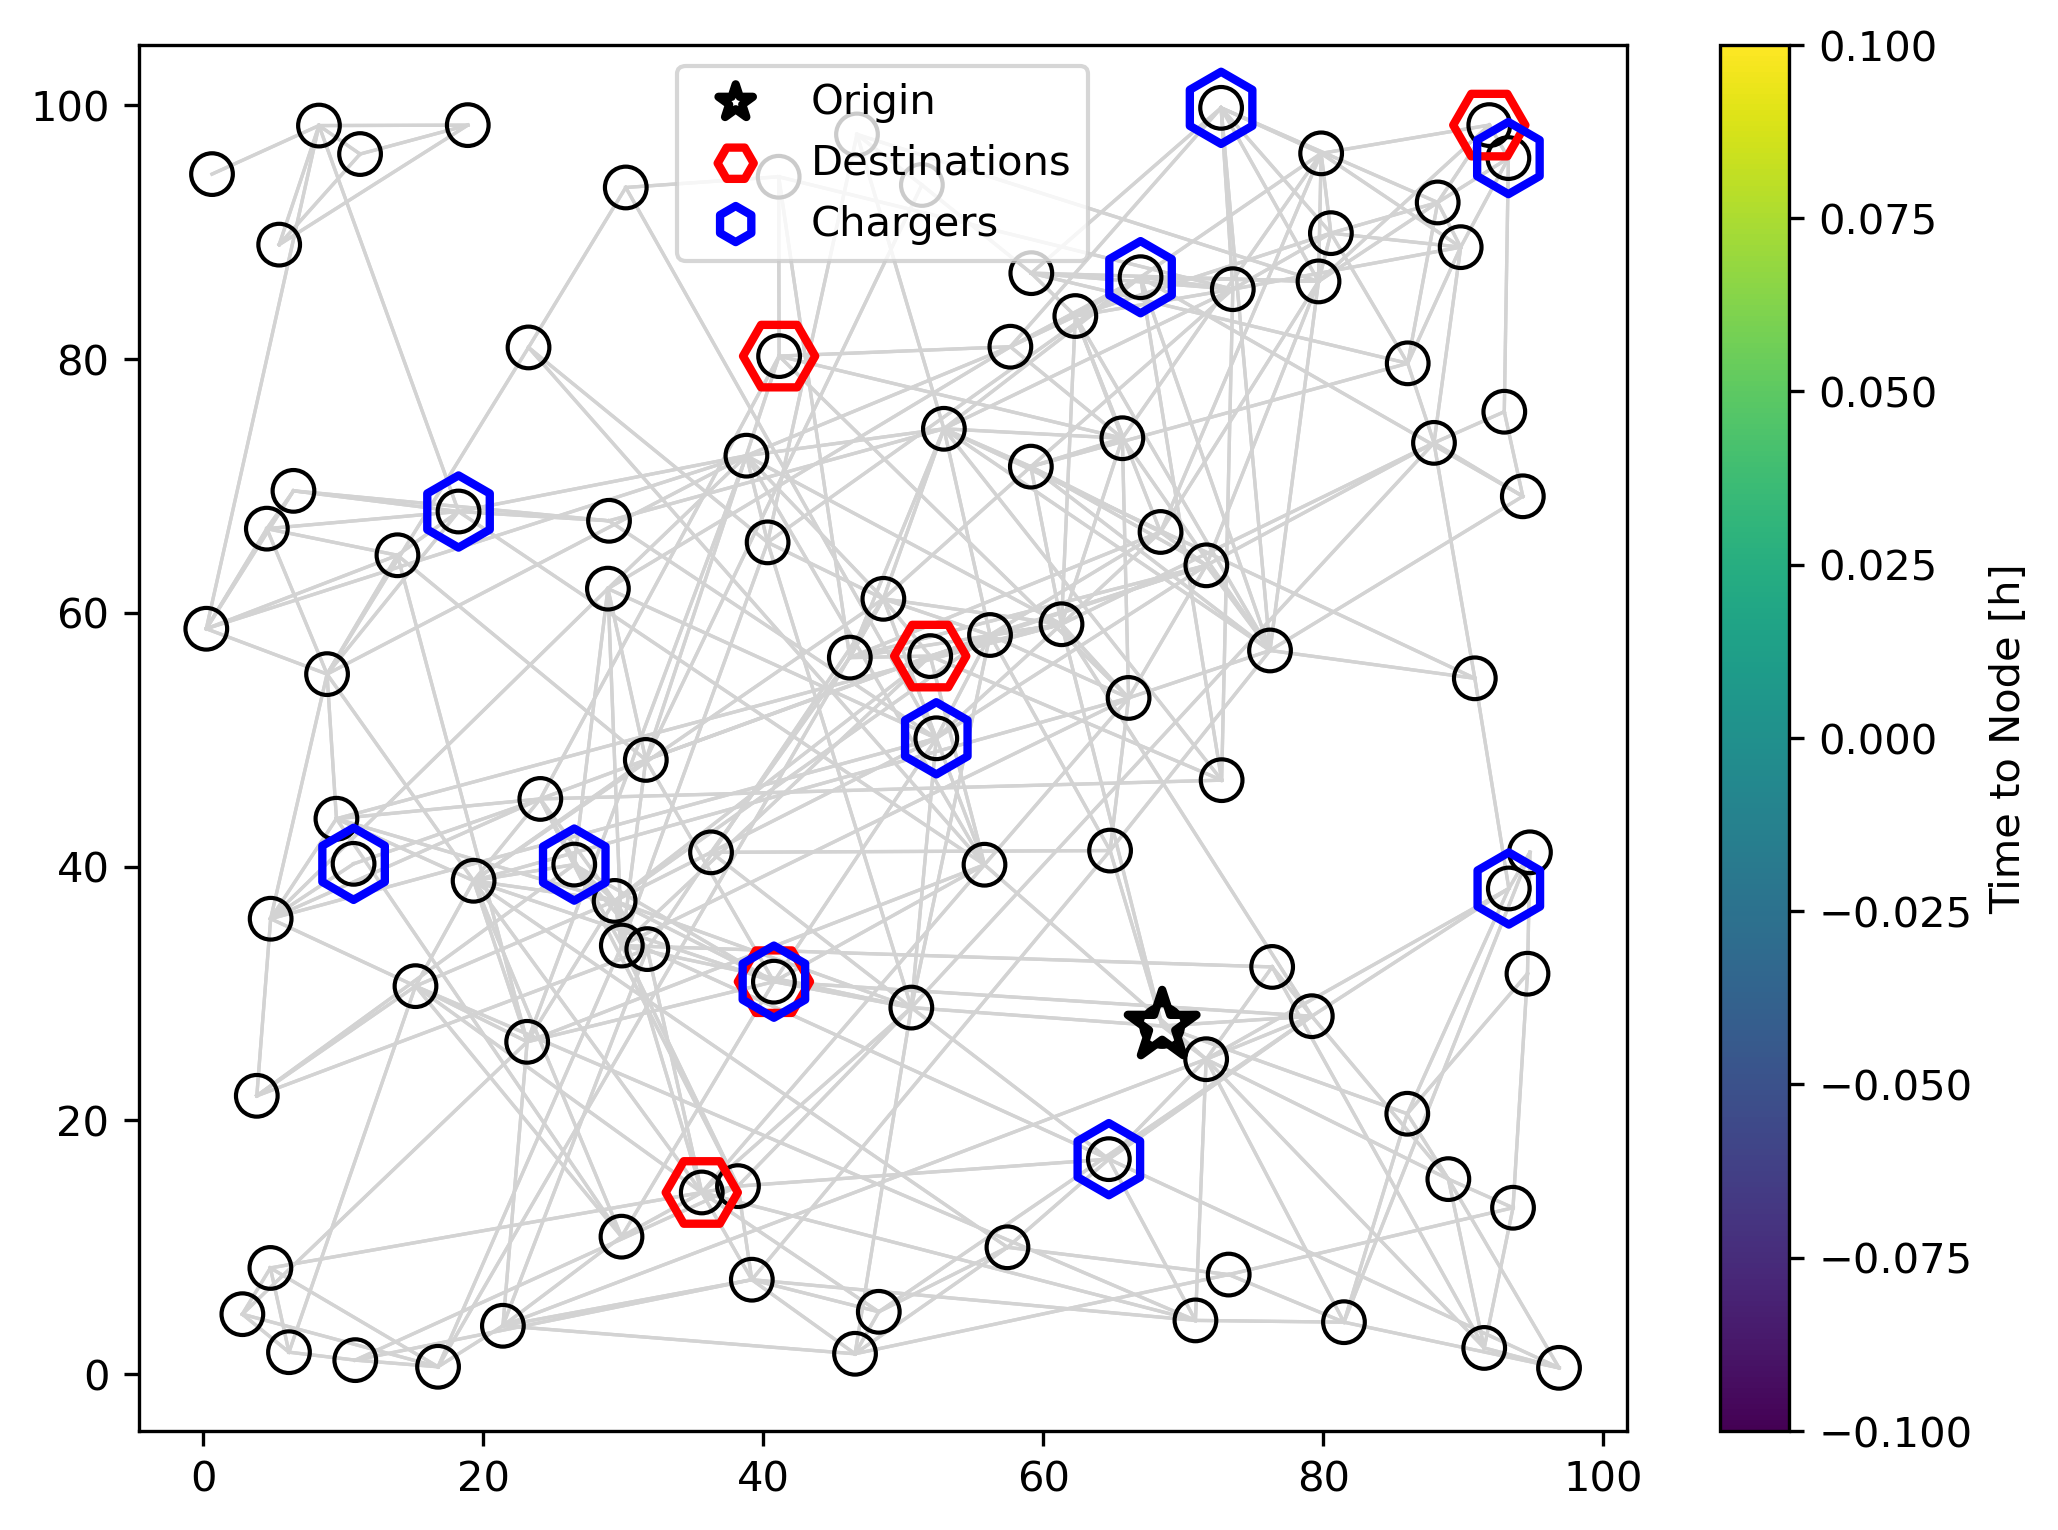
\includegraphics[width = \linewidth * 2 / 3]{figs/random_graph.png}
	\caption{Randomly generated graph with cardinality of 100 with 1 origin, 5 destinations, and 10 chargers.}
	\label{fig:random_graph}
\end{figure}

The links are traversed at speeds randomly selected from $\{35, 55, 90, 105\}$ kph. Like a real road network, all nodes are connected to the \gls{gcc} but not directly to all others. Because the random graph is based on nodes drawn from a uniform random distribution, the distances between nodes should be normally distributed. Because the probability of a given link is a function of distance, one would also expect the nodes in the middle to have the highest valency and for valency to be Poisson distributed and this is, indeed, the case.

\subsection*{California Graph}

The state of California contains 1,618 towns and cities, collectively referred to as places, per the US Census Bureau and 1,906 public DC charging stations per \gls{afdc}. Itineraries entirely contained in California will originate and terminate at California places. If additional range is needed beyond the remaining range at the start of the trip, \glspl{ev} will utilize one of the DC charging stations. The places and stations are completely connected by roads. Thus, an entity atlas can be computed by routing from each entity to each entity. For the purposes of reducing computation time and memory requirements, a limit on link ranges can be implemented which may result in a non-completely-connected entity atlas which should, nevertheless, be entirely contained within the \gls{gcc}. The components of the California entity atlas are shown in Figure \ref{fig:california_entity_atlas}.

\begin{figure}[H]
	\centering
	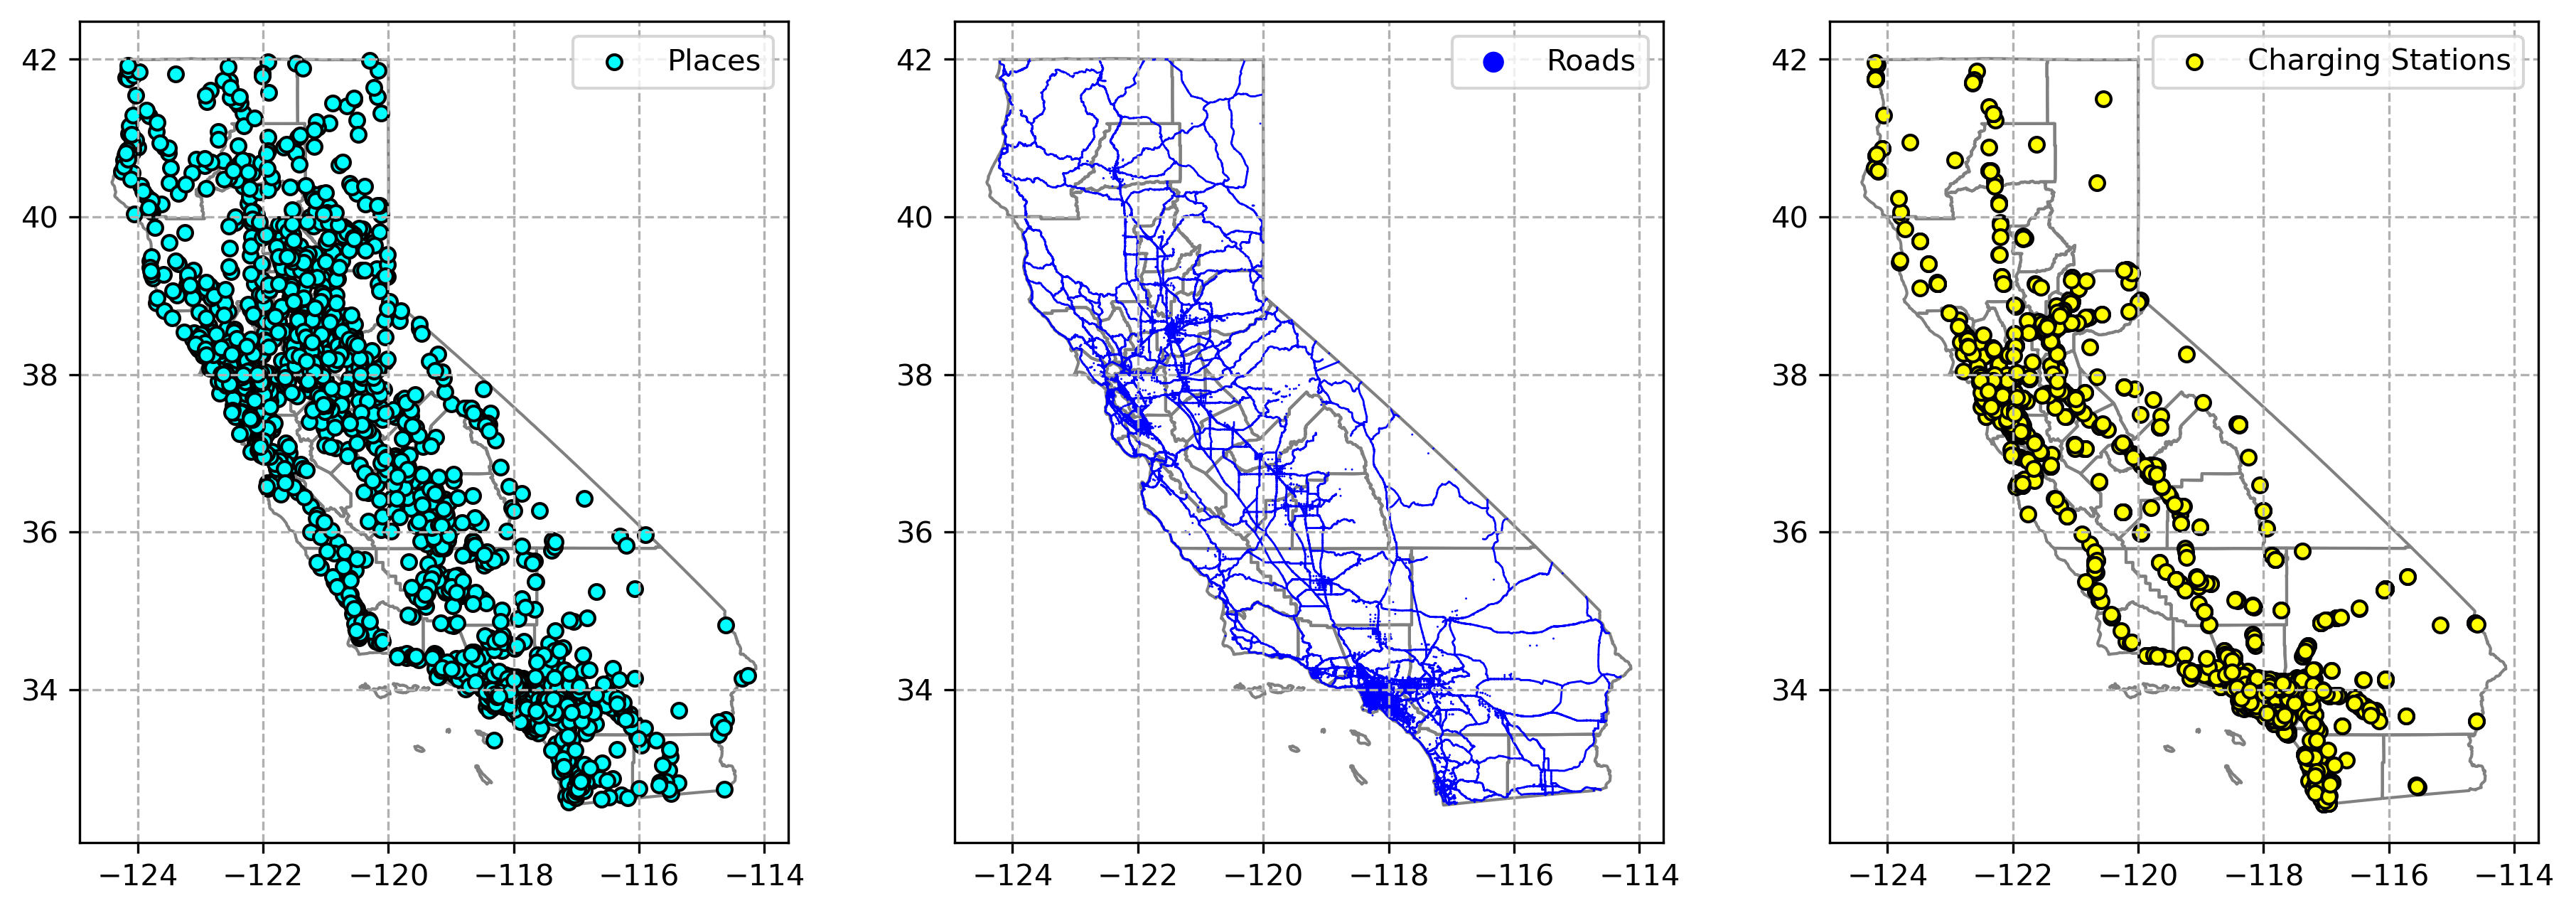
\includegraphics[width = \linewidth]{figs/California_Places_Chargers.png}
	\caption{Components of California entity atlas}
	\label{fig:california_entity_atlas}
\end{figure}